%%%%%%%%%%%%%%%%%%%%%%%%%%%%%%%%%%%%%%%%%%%%%%%%%%%%%%%%%%%%%%%%%%%%%%
% Summary of academic paper named ``A Wavelet-Based ECG Delineator: 
% Evaluation on standard databases"
% Prepared by Akshai M, ICFOSS on 7th February 2018
% CC-BY-SA 4.0, Free to use, learn, modify and distribute.
%%%%%%%%%%%%%%%%%%%%%%%%%%%%%%%%%%%%%%%%%%%%%%%%%%%%%%%%%%%%%%%%%%%%%%
\documentclass[twocolumn,showpacs,%
  nofootinbib,aps,superscriptaddress,%
  eqsecnum,prd,notitlepage,showkeys,10pt]{revtex4-1}
  

\usepackage{amssymb}
\usepackage{amsmath}
\usepackage{graphicx}
\usepackage{dcolumn}
\usepackage{hyperref}
\usepackage{titlesec}
%\titlespacing{\subsection}{0pt}{\parskip}{-\parskip}
\titlespacing{\subsection}{0pt}{1.1\baselineskip}{\baselineskip}
\titlespacing{\section}{0pt}{1.1\baselineskip}{\baselineskip}
%\titlespacing\section{0pt}{12pt plus 4pt minus 2pt}{0pt plus 2pt minus 2pt}
%\titlespacing*{\section}{0pt}{1.1\baselineskip}{\baselineskip}
\titlespacing{\paragraph}{0pt}{0pt}{.5em}[]

\begin{document}

\title{Summary of academic paper named ``A Wavelet-Based ECG Delineator: Evaluation on standard databases" }
\author{Akshai M}
\affiliation{Research Assistant, ICFOSS}

%\begin{abstract}

%\end{abstract}

\maketitle

\section{Introduction}
This document is a summary of the academic paper on the usage of wavelet transformation to detect fiducial points on ECG signal (QRS complexes, P and T waves) obtained from a single-lead electrocardiography.
\section{Chapters}
This summary is composed of four chapters namely Discrete Wavelet Transform, QRS detection, QRS Delineation, P and T waves Detection and delineation Techniques.
\label{sec:examples}
\subsection{Discrete Wavelet Transform}
Wavelet transform is obtained by multiplying a given signal with a wavelet analysing function.A wavelet is a rapidly decaying wave like oscillation with zero mean IE it exists in finite duration. Wavelet transformation decomposes the signal as a combination of a set of basis functions, obtained through scaling and translation of a prototype wavelet.Wavelet transform of a signal x(t) is \\ \\
\begin{math}
W_ax(b) = \frac{1}{\sqrt[]{a}}\int_{-\infty}^{+\infty}x(t)\psi \left ( \dfrac{t-a}{b}\right ) dt , a > 0
\end{math}
\\
\\
where a is the scaling factor and \( \psi (t) \) is the prototype wavelet.
\\
ECG is composed of slopes and local maxima (or minima) at different scales, occurring at different time instants within the cardiac cycle. If the prototype wavelet \( \psi (t) \) is made derivative of a smoothing function say \( \theta (t)\)the detection would be made easier. Wavelet transform of a signal x(t) may now be defined as \\ \\
\begin{math}
W_ax(b) = -a \frac{d}{db}\int_{-\infty}^{+\infty} x(t) \theta_a (t-b) dt
\end{math}
\\
\\
where \( \theta_a(t) = \left (\frac{1}{\sqrt[]{a}} \right ) \theta \left ( \frac{t}{a} \right ) \) , which is the scaled version of smoothing function.
\\
Discrete Wavelet Transform (DWT) is computed by passing a signal  successively through a high pass and a low pass filter. For each  decomposition level, signal convolve with low pass filter H(z) and with high pass filter G(z). The signals would be continuously separated into low frequencies and high frequencies as shown in Fig.2.

\begin{figure}
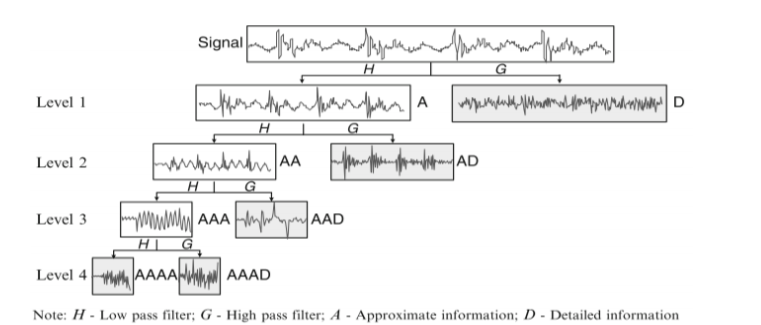
\includegraphics[width=0.5\textwidth]{fig1.png}
\caption{\label{fig:fig1} DWT Process  }
\end{figure}

\begin{figure}
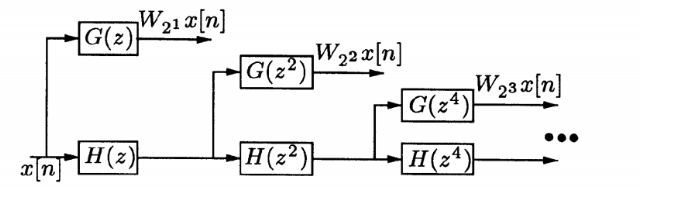
\includegraphics[width=0.5\textwidth]{fig2.png}
\caption{\label{fig:fig2}Algorithme \`a  trous.  }
\end{figure}
The scaling factor \(\mathbf{a} \)  and/or translation parameter \( \mathbf{b} \) may be discretised based on a dyadic grid on time scale plane to obtain dyadic discrete wavelet transform as shown below.Dyadic wavelet transforms are scale samples of wavelet transforms following a geometric sequence of ratio 2. Assuming a = \(2^k\) and b= \(2^k l \) \\ \\
\begin{math}
\psi_{k,l}(t) = 2^{-k/2} \psi \left (  2^{-k} t-l\right ); k, l \in Z^+.
\end{math} \\ \\
This discrete transformation is equivalent to a filter bank composed of cascaded Finite impulse response filters. The cascading of filters make the signal time-variant and reduce the temporal resolution for increasing scales. To preserve the time-invariance and temporal resolution same sampling rate is used in all scales using a technique called algorithme \`a  trous. Fig 2 represents the algorithm with coefficients \( W_2^{k}x[2^kl] \)The equivalent frequency response for kth scale can be represented as 
\\ 
\\
\begin{math}
Q_k \left ( e ^ {jw} \right ) = \begin{cases} G (e^{jw}) & \text{k=1} \\ G(e^{j2^{k-1}w} ) , \prod_{l=0}^{k-2}H(e^{j2^lw}) & \text{k} \geq 2 \end{cases}
\end{math}
\\
\\ \\
The paper suggests usage of 4th degree spline prototype wavelet as follows
\\ \\
\begin{math}
\theta (\Omega) =  \left ( \frac{\sin(\Omega/4)}{\Omega/4} \right ) ^ 4
\end{math}
\\ \\ 
whose Fourier transform is given by \\
\begin{math}
\Psi (\Omega) = j \Omega \left ( \frac{\sin(\Omega/4)}{\Omega/4} \right ) ^ 4
\end{math}
\\
\begin{figure}
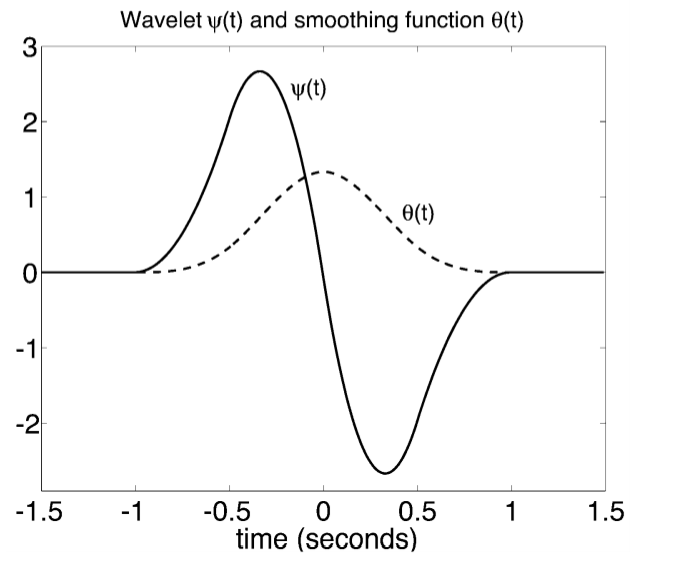
\includegraphics[width=0.5\textwidth]{fig3.png}
\caption{\label{fig:fig3} Prototype wavelet \( \psi (t) \) \(\theta (t) \) }
\end{figure} 
%Figure
\begin{figure}
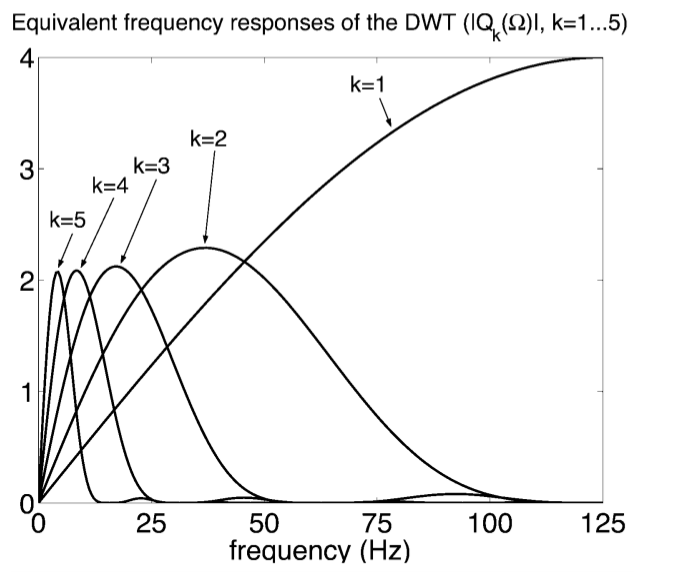
\includegraphics[width=0.5\textwidth]{fig4.png}
\caption{\label{fig:Fig4} Equivalent Frequency responses of DWT at scales \(2^k , k = 1, .., 5 \)   }
\end{figure}
Fig 3 represents the prototype wavelet and smoothing function.FIR filters , H(z) and G(z), to implement DWT may be derived as as 
\\ \\
\begin{math}
H(e^{jw}) =  e^{jw/2} \left ( \cos (w/2)\right ) ^3 \\
G(e^{jw}) =  4je^{jw/2} \left( \sin(w/2) \right )
\end{math}
\begin{figure}
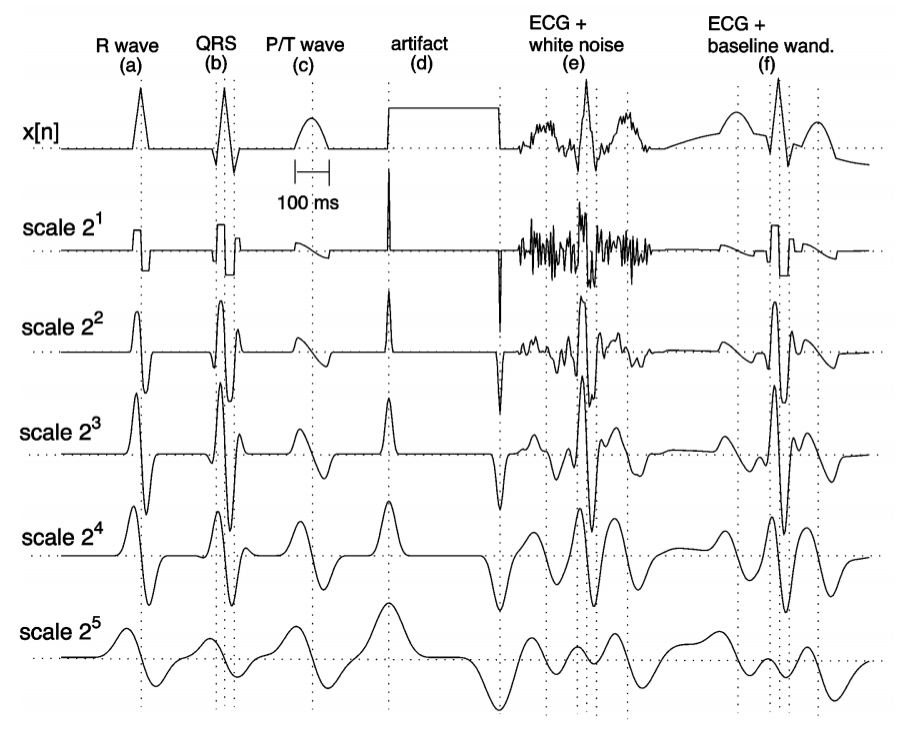
\includegraphics[width=0.5\textwidth]{fig5.png}
\caption{\label{fig:Fig5} WT of first five scales of ECG-like simulated waves   }
\end{figure}
\\ \\
Using algorithme \`a trous the frequency responses of first five scales are represented on Fig 4.To obtain frequency responses for sampling rate other than 250Hz, a new set of filters having equivalent analogue frequency responses similar to what shown in Fig 4 are used. \\

\subsection{QRS Detection}
From Fig 4, we can conclude that most of the energy of the ECG signal lies within scales \( 2^1 \) to \( 2^ 5\). QRS values are really low on scales higher than \( 2 ^ 4 \). Fig 5 shows simulated waves similar to ECG. QRS complexes are detected through searches across scales for ``maximum modulus lines'' exceeding a preset threshold at scales \( 2^1 \) to \( 2^ 4\). The zero crossing of WT at a scale \( 2^1 \) between a positive maximum-negative minimum pair is marked as QRS. The detection is not restricted to R wave, but also allows detection of negative waves as well.
\subsection{QRS Delineation}
Delineation algorithm looks for start and end of envelope on  \( 2^2 \) scale for significant maxima , which is local maximum modulus above the threshold defined by previous or subsequent waves. The zero crossings are then assigned on \( 2^1 \) scale to name the waves in all possible QRS morphology.
\subsection{T and P wave detection and Delineation}
T wave detection happens in a search window relative to the QRS position and recursively computed R-R interval. The algorithm looks for local maxima on  \( 2^4 \) scale and if at least two exceeds the local threshold then it is marked as a T waves and is named based on the number and polarity of the found maxima.
P wave detection algorithm is similar to that of T wave detection. Recursively calculated R-R search window and adequate thresholds are used to detect the waves.

%\subsection{Validation of results}
%MIT-BIH Arrhythmia database, QT , European ST-T database and dataset 3 of CSEDB were used to validate the results.
%For validation of QRS detection , MITDB, EDB and QTDB were used. To evaluate delineation performance QTDB and CSEDB were used. QRS detector sensitivity \( S_e=TP/\left ( TP +FN \right ) \)and positive predictability  \( P^+=TP / \left ( TP + FP \right )\) was calculated. TP is the number of True positive detections, FN represents false negative detections while FP represents false positive detections. The QRS detector attained 43 FP and 23 FN of 14,841 analysed beats ( \( S_e\) = 99.84\% and \( P^+\) =99.70\% based on excerpts used by other existing WT based detectors and proposed WT approach was found to be better.

%\section{Conclusion}
%WT based ECG delineation algorithm was validated on several annotated databases with varying sample rates and was found to outperform existing algorithms  with errors well within observed inter cardiologist variations. The algorithm provides large improvement in terms of T wave detection and delineation. Dynamic multi scale approach was found to attenuate noises better and with great temporal resolution. The process however could have been better validated for different morphologies if more number of annotations we available for single-lead ECG signals.



\end{document}